\documentclass[11pt]{letter}
\usepackage[utf8]{inputenc}
\usepackage{geometry}
\usepackage{graphicx}
\usepackage{fancyhdr}

\usepackage[colorlinks=true]{hyperref}
\hypersetup{
    pdftitle={Cover Letter},
    pdfauthor={Leonardo Uieda},
    linkcolor=black,
    citecolor=black,
    filecolor=black,
    urlcolor=black
}

\longindentation=0pt

% Redefine the empty style so the front page also has a header.
\fancypagestyle{empty}{ %
    \fancyhf{} % remove everything
    \lhead{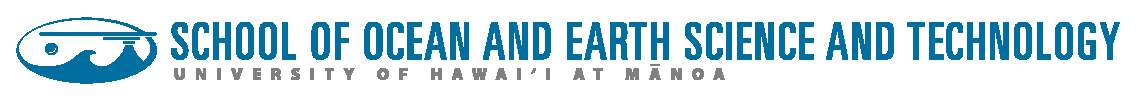
\includegraphics[width=\columnwidth]{images/soest-logo.eps}}
    %\lhead{\includegraphics[width=0.5\columnwidth]{images/uh-logo.eps}}
    \cfoot{\thepage}
    \renewcommand{\headrulewidth}{0pt}
    \renewcommand{\footrulewidth}{1pt}
    \setlength\headheight{31pt}
}
\pagestyle{empty}

\signature{ Leonardo Uieda }
\address{
    1680 East-West Road, POST 804
    \\
    Honolulu, HI 96822, USA.
    \\
    email: \href{mailto:leouieda@gmail.com}{leouieda@gmail.com}
    \\
    phone: +1 808 428 4521
}

\begin{document}

\begin{letter}{
    Department of Statistics
    \\
    Faculty of Science
    \\
    3182 Earth Sciences Building, 2207 Main Mall
    \\
    Vancouver, BC Canada V6T 1Z4
}
\opening{Dear Members of the Search Committee:}

I am writing to apply for the position of Lecturer in the Masters of Data
Science Program of the University of British Columbia, as advertised on the
Department of Statistics website.
I am a visiting research scholar at the University of Hawai'i in the Department
of Geology and Geophysics.
My research interests include geophysical inverse problems, scientific
software development, and geospatial data visualization.

% Research and OSS
My research training is in developing methods and algorithms for solving
geophysical inverse problems.

The methods that I developed during my Masters and PhD are computationally
efficient solutions to the problem of inferring subsurface density variations
from observation of distances in the Earth's gravity field.

I created software to support my research and that of my lab.

The software Tesseroids (link) and Fatiando a Terra (link).


I have been developing open-source software in Python for the past decade.
All of my software projects are on Github.

SOMETHING ABOUT THE PROJECTS.
HOW THEY USE GITHUB AND MODERN PRACTICES.


SOMETHING REPRODUCIBLE SCIENCE AND THE PINGA LAB TEMPLATE.

My research training is in geophysical inverse problems.

% Teaching

Before starting my current position, I worked for three years as assistant
professor at the State University of Rio de Janeiro (UERJ), Brazil.

There, I taught undergraduate-level classes on geophysical methods,
introduction to geology, and programming and numerical methods.

I had the opportunity to create the Geophysics I and II and the Programming
and Numerical Methods courses.

All rely heavily on Jupyter notebooks, numerical simulations, and real world
datasets.

My geophysics classes make use of Jupyter notebooks coupled with Fatiando a
Terra to provide the students with an interactive environment for exploring a
given topic.

Each class module includes a notebook with interactive simulations and/or real
data to help guide the students through a series of formative and summative
assessments.

My programming course is entirely implemented as Github repositories using
Github Classroom.
Each module has a repository with a group project.
The students submit their work as git repositories (e.g., the projects for the
2016 class are at https://github.com/mat-esp-2016) and the grading and feedback
are provided in Github issues (e.g.,
https://github.com/mat-esp/about/issues/259).
This workflow allowed me to manage a project-based class with over 70 students
as the sole instructor.

I have also taught short workshops on Python programming and geophysics.

All of my teaching material is available on Github with links and descriptions
on my personal website http://www.leouieda.com/teaching/.


% Conclusion

I am excited bla bla bla

With my research and teaching experience, I would feel comfortable teaching a
range of classes from the MDS program, including
programming, data visualization, software development, regression, and machine
learning.

I am particularly interested in the Data Science Workflows class, a subject in
which I have been recently working on
(http://www.leouieda.com/blog/paper-template.html).

Collaborate on the Capstone projects and possibly bring in problems from Oil
and Gas and mining industries.

I can bring the experience of a different field to the data science program.

I intend to continue my research program with external collaborators.

I would like to collaborate with colleagues from the Data Science Lab to solve
interesting problems in Geophysics and Data Science.

I would also like to connect the Department of Statistics with specialists in
geophysical inversion from the Earth Sciences like Oldenburg and Haber.


\closing{Thank you for your consideration,}

\end{letter}

\end{document}
